% Template for ICASSP-2013 paper; to be used with:
%          spconf.sty  - ICASSP/ICIP LaTeX style file, and
%          IEEEbib.bst - IEEE bibliography style file.
% --------------------------------------------------------------------------
\documentclass{article}
\usepackage{spconf,amsmath,graphicx}

% Example definitions.
% --------------------
\def\x{{\mathbf x}}
\def\L{{\cal L}}

% Title.
% ------
\title{A Cross-platform, Standalone Application for Audio Retrieval by Rhythmic and Timbral Similarity}
%
% Single address.
% ---------------
\name{Aneesh Vartakavi, Cameron Summers} %\thanks{Thanks to XYZ agency for funding.}
\address{Georgia Tech. Center for Music Technology (GTCMT)}
%
% For example:
% ------------
%\address{School\\
%	Department\\
%	Address}
%

\begin{document}
%\ninept
%
\maketitle
%
\begin{abstract}
This paper details the implementation of a standalone desktop application in C++ for retrieval of audio files by rhythmic and timbral similarity, notable for being, to our knowledge, the first application of its type under the GNU General Public License (GPL). The implementation focuses on audio loops - short audio files intended to restart immediately upon completion for compositional purposes - to address the difficulty of navigating large loop libraries manually. The audio similarity measure utilizes tempo detection and statistical features of spectral frame periodicity to provide a ranking of most similar audio files to a particular reference file. Although similarity measures are somewhat subjective and difficult to evaluate, we propose two evaluations: 1) A classification accuracy on a ground truth data set developed by the authors using real-world audio loops and 2) A synthetic ground truth data set developed by the authors using related beat patterns at different tempos that demonstrates tempo invariance in retrieving rhythmically similar audio. (HOW ABOUT ONE LINE HERE TALKING ABOUT THE FINAL OUTCOME?)
\end{abstract}
%
\begin{keywords}
audio similarity, audio retrieval, distance matrix, beat spectrum, tempo detection, C++, JUCE
\end{keywords}
%
\section{Introduction}
%\label{sec:intro}

With advances in technology, large libraries of audio loops on a single hard drive have become commonplace. Navigating these libraries becomes increasingly difficult because knowledge about the files must be manually tagged or inspected by ear. A computational approach to audio retrieval via a similarity measure dramatically reduces the time spent navigating these libraries.

In this paper, we detail an implementation of a standalone desktop application in C++ for retrieval of audio loops by rhythmic and timbral similarity. A common task is finding an audio sample to sound simultaneously or in succession with a particular reference sample. The application allows a user to filter loops outside an acceptable range of tempo along with rhythmic and timbral distance given a particular reference loop. The tempo detection uses a simple approach based on characteristics of audio loops and the rhythmic distance is based on features derived from spectral periodicity. The timbral measure is based on euclidean distance between features derived from the Mel Frequency Cepstral Coeffecients (MFCC).

Our software provides the user with an interface to query for similar loops using a slider interface to specify a range of tempo, timbral and rhythmic distances. We believe this application has the potential to significantly reduce the amount of time spent searching a large database for similar loops.

\section{Related Work}

Several studies exist on audio retrieval by rhythmic similarity using statistical features since this approach requires limited or no human input to operate. One successful instance uses correlated energy peaks across frequency sub-bands \cite{scheirer1998tempo}  while another uses a feature vector from a low frequency-weighted Short-Time Fourier Transform (STFT) \cite{wold1999classification}. Another approach using spectral periodicity called the Beat Spectrum \cite{foote2001beat} is utilized for rhythmic similarity in this application, because it is based on self-similarity of the audio, no particular features are required of the audio such as silence or periodic energy peaks - Only repetitive events are required, which are common in audio loops. We derive a periodicity measure from the similarity matrix similar to \cite{foote2001beat} for our application.

MFCC based timbre space has been found to be a good model for perceptual timber space \cite{terasawa2005thirteen}. MFCCs have since been used to create similarity measures \cite{jensen2009quantitative} for genre recognition \cite{levy2006lightweight}, \cite{jensen2006evaluation}. We derived a simple timbral distance measure based on the euclidean distance between a feature vector derived from the MFCC's.

Several closed-source applications exist for determining audio similarity in libraries of audio files such as \textit{Similarity} \cite{similarityapp}. However, \textit{Similarity} and most others are meant primarily for file library organization (e.g. removing duplicate files) and not for rapid navigation for compositional purposes. Another open-source command line application under a BSD-style license written in Python, AudioCompare \cite{audiocompare}, utilizes indices of dominant frequencies of the STFT for a general similarity measure, but this is not a musically descriptive measure and unreliable for our use case. 


\section{Methodology}

In this section, we describe the implementation of our algorithm, particularly the tempo estimate, rhythmic similarity and the timbral similary measure. We also briefly discuss a GUI implementation to navigate a library using the aforementioned measures.

\subsection{Tempo Estimation}
WHAT DO YOU THINK ABOUT SEPARATING TEMPO ESTIMATION AND RHYTHMIC SIMILARITY?

We were going to say that the rhythmic similarity is tempo invariant, so I think we should separate the two. I'm fine with whatever you decide in the end.


\subsection{Rhythmic Similarity}

The rhythmic similarity recommendation algorithm is composed of two primary components that can be applied together or independently in the application: tempo estimation and distance between feature vectors of the spectral periodicity. For tempo estimation of an audio file, we use a simple method shown in equation (\ref{eq:tp}) where \(T\) is the tempo, \(n\) is the number of expected beats in the loop, \(f_s\) is the sampling frequency of the audio, and \(N\) is the number of samples. This method is based on an assumption that the length of the audio loops in beats will always be a power of 2 of a 4/4 measure - a group of 4 beats - which is generally true for many loop libraries. Additionally, we scale the tempo to a range of 50-160 beats per minute.

\begin{equation}
\label{eq:tp}
T = 60 * n * f_s * 1/N
\end{equation}

While there can be errors with this method when the assumptions do not hold, it worked consistently well for the real-world EarSketch \cite{earsketch} loops used for evaluation.

The second component of rhythmic similarity comes from a calculation of statistical features of spectral periodicity, called the Beat Spectrum by \cite{foote2001beat} who provides a detailed overview. We calculate the spectral periodicity as described in \cite{foote2001beat} and include some processing steps prior to computing features. The spectral periodicity of an audio file is derived from a similarity matrix S where \(S_{ij}\) is the cosine distance between the STFT of i-th and j-ith block of the audio file. A block size of 1024 and hop size of 512 were used for the STFT. At a typical sampling frequency of 44100Hz for the audio loops we tested, this provides resolution in time of 23ms, which is sufficient for detecting rhythms even at faster tempos that adequately describe the audio file. Variations on these values could be tested in future research to determine if optimization is possible.

Next each super diagonal of S is summed as in equation (\ref{eq:bs}) to give a representation of the spectral periodicity in the lag domain, where l is lag and k is the block index. An example of the result is shown in Fig. \ref{fig:bs1_pre}, where the periodicity of events in the audio is evident. Alternatively, the spectral periodicity can be viewed as an autocorrelation of a vector of elements where each element is the STFT of a block of samples in the audio file.

\begin{figure}[h!]
	
  \centering
    \centerline{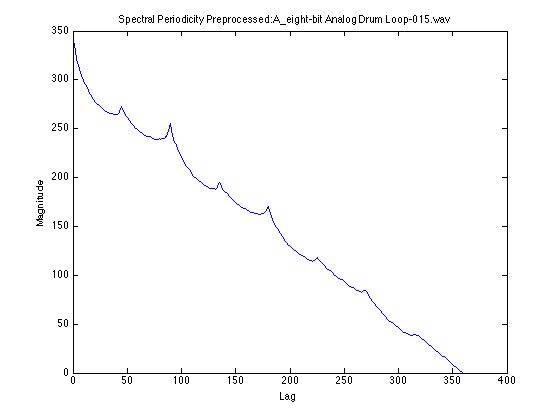
\includegraphics[width=0.5\textwidth]{bs_pre.png}}
     \caption{Spectral periodicity measure for a sample loop}\label{fig:bs1_pre}
\end{figure}

\begin{equation}
\label{eq:bs}
SP(l) = \sum S(k, k+l)
\end{equation}

In the implementation in application, the spectral periodicity was calculated using a single similarity matrix with a length equal the number frames in the entire audio file. The audio file could alternatively be segmented and the spectral periodicity calculated on each segment as described by the Beat Spectrogram in \cite{foote2001beat}, but since audio loops are often taken as a single unit for the compositional use case, our approach seems more appropriate for the application. Future implementations might explore this alternative and compare the performance for similarity ranking.

Prior to calculating features on spectral periodicity signal some preprocessing steps were taken to increase robustness of the measure. First, since the spectral periodicity is an autocorrelation and the number of elements summed decreases as the lag increases, a line was fit using least squares and subtracted from the signal. Next, the signal was normalized and inverted so that lags of lower distances had higher values by subtracting the signal from an equally long signal with every value a 1. Finally, a three point moving average filter was used for smoothing. Fig. \ref{fig:bs1_post} shows the post-processed signal.

\begin{figure}[h!]
 \centering
	\centerline{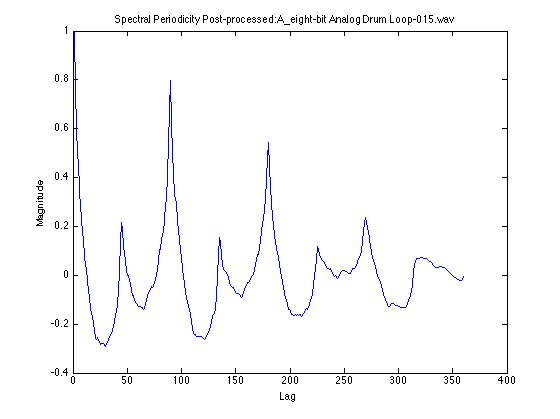
\includegraphics[width=0.5\textwidth]{bs_post.png}}
      \caption{Spectral periodicity measure after pre-processing}	\label{fig:bs1_post}
\end{figure}

After the preprocessing steps, a feature vector was constructed to describe the signal and these features were standardize by removing the mean and dividing by the standard deviation of each feature. A list of these features are shown in Table \ref{tab:bs_feat}. Lastly, the algorithm determines a rhythmic distance measure by calculating the euclidean distance between spectral periodicity feature vectors of two audio files.

\begin{table}[h!]
  \begin{center}
    \begin{tabular}{| p{7.0cm} |}
    \hline
    Line Slope (LS) \\
    \hline
	LS y-intercept\\
	    \hline
	Instaneous values at beats (assuming 4/4) \\
	    \hline
	Standard Deviation \\
	    \hline
	Skewness \\
	    \hline
	Kurtosis \\
	    \hline
	Sum of absolute value of difference between LS line and signal \\
	    \hline
	Number of changes in signal slope \\    \hline
    \end{tabular}
  \end{center}
  \caption{Features Derived from Spectral Periodicity}\label{tab:bs_feat}
\end{table}
    

\subsection{Timbral Similarity}

The timbral distance measure was based on thirteen dimensional MFCCs, which were computed as described in \cite{jensen2009quantitative}. Additionally, we also computed the first derivative of the MFCC coefficients, storing a 52 dimensional feature vector of the mean and standard deviation of the MFCCs and their derivatives for each audio file. The timbral distance measure was formulated as the Euclidean distance between the aforementioned feature vector.

\subsection{Implementation}

Processing spectral periodicity features on large libraries of files requires speed and this informed the application design decisions. We chose the C++ framework JUCE \cite{juce} because C++ code can be optimized efficiently for time and memory and JUCE is highly regarded in the audio software development sphere for its user interface styling and audio utilities. Additionally, JUCE allows for multi-platform development and deployment, making greater the potential future dissemination of the application. We also use the Eigen Library\cite{eigenweb}, which provides optimized linear algebra routines and an FFT wrapper.

\subsection{User Interface}
Given the difficulty of navigating large loop libraries, the user interface of the application seeks to assist the algorithm in making this process simple and fast. A user can select a reference file in a list box on the left on which to compare other files in the library and has the option of listening to that file. Next there are three range sliders available; one for tempo, one for rhythmic distance and one for timbral distance. Then Similar files are automatically shown or removed in the right box according to the slider positions and those can also be played back by the user. A screenshot of the application is shown below in Fig. \ref{fig:gui}. The application also writes previously calculated features for a directory in a cache and allows the user to load and reuse that cache to avoid calculating features on the directory again. The cache, however, forces a re-computation when files are changed within the directory.

\begin{figure}[h!]
  \centering
    \centerline{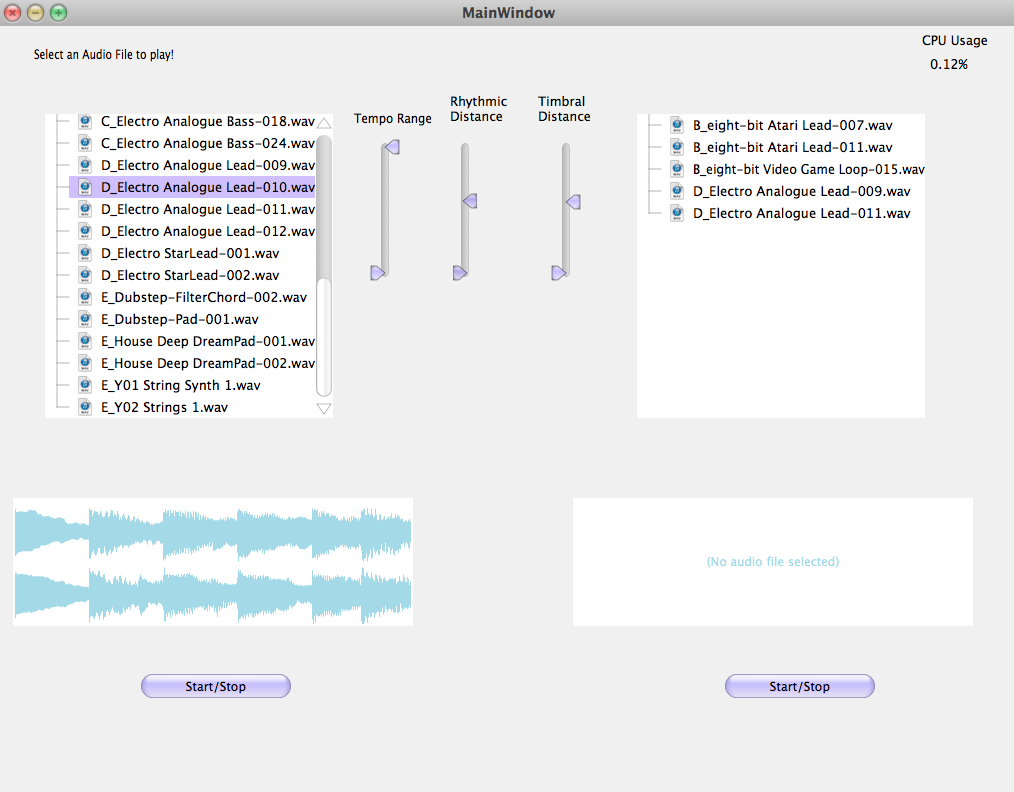
\includegraphics[width=0.5\textwidth]{fLoop_gui.png}}
      \caption{Application GUI Screenshot}\label{fig:gui}
\end{figure}

\section{Evaluation}
We propose two methods for evaluation rhythmic similarity functions implemented in the application. Unable to find an accepted ground truth dataset for rhythmic similarity, the authors developed a ground truth set by selecting manually 30 loops from the EarSketch library and separating them by ear into 5 distinct rhythmic classes each with 6 loops. For each loop L, distances were calculated to the other 29 loops and ordered from the least distance to greatest. Then for each of the smallest K distances an accuracy was recorded as the number of loops matching the class of L divided by K. Fig. \ref{fig:eval1_dist} shows the ordered distances and associated classes for one audio loop in the ground truth seen in the figure as the loop with a distance of zero.

\begin{figure}[h!]
  \centering
   \centerline{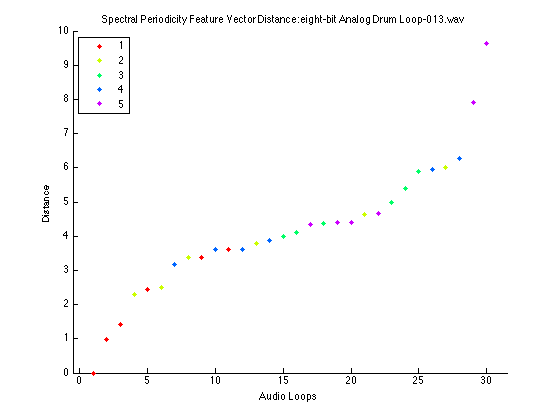
\includegraphics[width=0.5\textwidth]{distance_graph_eval1.png}}
      \caption{INSERT CAPTION}\label{fig:eval1_dist}
\end{figure}

Table \ref{tab:bs_eval} shows the average accuracy for all 30 loops for varying K. In other words, the top recommended loop was of the same class as the reference loop 80\% of the time.

\begin{table}[h!]
  \begin{center}
    \begin{tabular}{| c | c | c | c | c |}
    \hline
    K=1 & K=2 & K=3 & K=4 & K=5 \\
    \hline
    80\% & 70\% & 66\%  & 57\% & 55\% \\
    \hline
    \end{tabular}
  \end{center}
  \caption{Average Class Accuracies}\label{tab:bs_eval}
\end{table}

A second evaluation for tempo detection used the same 30 loops from the EarSketch library for which the loops had 7 unique tempos. The tempo detection accuracy for these 30 loops was 29 correct out of 30, or 97\%, and the single incorrectly calculated tempo was off by 1 bpm.


\section{Discussion}

The objective of providing a user a computational approach to and software application for navigating a loop library was fairly successful. As seen in Table 1 the most highly recommended loop was of the same classes as the reference loop 80\% of the time. From the standpoint of the user, this significantly reduces the time spent looking for a similar loops that may complement one another musically. Care must be taken though, because although the authors have musical training, biases or inaccuracies may exist in the ground truth data. A more comprehensive future evaluation might include multiple ground truths from different musicians and loop libraries.

The tempo detection method works quite well in testing as indicated by the 97\% accuracy in detecting the tempo on the ground truth. However, the assumption that any loop in a large library is a multiple of a power of 2 of a 4/4 measure may not always hold in real-world cases. The loop may be slightly longer or shorter, as is likely the case in the single incorrectly calculated tempo in the previous section, or in 3/4 time and small changes such as this make a large impact in selecting loops to form a composition. Since the user interface allows for a variable range in tempo, the user has significant flexibility in overcoming shortcomings such as this. Future implementations of tempo detection would likely benefit from a more robust system.

Future work could include several improvements to the existing algorithm and application. For example, additional features could be calculated and principal component analysis could be used to determine the most useful features. Additional similarity components could added such as chroma-based key detection since the knowledge of key would be quite useful for this use case. And other user interfaces such as self-organizing maps of the audio library may yield intuitive and creative ways for composers to select loops for a composition.


% Below is an example of how to insert images. Delete the ``\vspace'' line,
% uncomment the preceding line ``\centerline...'' and replace ``imageX.ps''
% with a suitable PostScript file name.
% %-------------------------------------------------------------------------
%\begin{figure}[htb]

%\begin{minipage}[b]{1.0\linewidth}
%  \centering
%  \centerline{\includegraphics[width=8.5cm]{image1}}
%  \vspace{2.0cm}
%  \centerline{(a) Result 1}\medskip
%\end{minipage}
%
%\begin{minipage}[b]{.48\linewidth}
%  \centering
%  \centerline{\includegraphics[width=4.0cm]{image3}}
%  \vspace{1.5cm}
%  \centerline{(b) Results 3}\medskip
%\end{minipage}
%\hfill
%\begin{minipage}[b]{0.48\linewidth}
%  \centering
%  \centerline{\includegraphics[width=4.0cm]{image4}}
%  \vspace{1.5cm}
%  \centerline{(c) Result 4}\medskip
%\end{minipage}
%
%\caption{Example of placing a figure with %experimental results.}
%\label{fig:res}
%
%\end{figure}


% To start a new column (but not a new page) and help balance the last-page
% column length use \vfill\pagebreak.
% -------------------------------------------------------------------------
%\vfill
%\pagebreak

%\vfill\pagebreak

%\section{REFERENCES}
%\label{sec:refs}
% References should be produced using the bibtex program from suitable
% BiBTeX files (here: strings, refs, manuals). The IEEEbib.bst bibliography
% style file from IEEE produces unsorted bibliography list.
% -------------------------------------------------------------------------
\bibliographystyle{IEEEbib}
%\bibliography{strings,refs}
\bibliography{references}


\end{document}
